\documentclass[12pt,a4paper]{article}

% ==================== 中文支持 ====================
\usepackage[UTF8]{ctex}
\usepackage{geometry}
\geometry{left=2.5cm, right=2.5cm, top=2.8cm, bottom=2.8cm}

% ==================== 常用宏包 ====================
\usepackage{graphicx}
\usepackage{booktabs}
\usepackage{enumitem}
\usepackage{caption2}
\usepackage{float}
\usepackage{hyperref}
\usepackage{titlesec}
\usepackage{fancyhdr}
\usepackage{setspace}
\usepackage{amsmath}

% ==================== 页面设置 ====================
\onehalfspacing
\pagestyle{fancy}
\fancyhf{}
\fancyhead[C]{\small 北京印刷学院\,·\,"千人百村"实践调研报告}
\fancyfoot[C]{\thepage}
\renewcommand{\headrulewidth}{0.4pt}

% ==================== 标题格式 ====================
\titleformat{\section}{\large\bfseries}{\thesection、}{0pt}{}
\titleformat{\subsection}{\normalsize\bfseries}{（\thesubsection）}{0pt}{}

% ==================== 图片路径 ====================
\graphicspath{{figures/}}

% ==================== 文档信息 ====================
\title{
    \vspace{-1cm}
    {\LARGE\bfseries 数智赋能平谷传统渔业转型：\\[6pt] 基于四村实地调研的现状分析与路径探索}
}
\author{
    北京印刷学院\;"千人百村"实践队\;"数智渔韵"课题组 \\[4pt]
    \small 指导教师：\underline{\hspace{3cm}} \qquad
    课题组成员：\underline{\hspace{6cm}}
}
\date{2026\,年\,7\,月}

\begin{document}

% ==================== 封面 ====================
\maketitle
\thispagestyle{empty}
\vspace{2cm}
\begin{center}
\textbf{摘\quad 要}
\end{center}
\vspace{0.3cm}

\noindent 乡村振兴战略背景下，北京市平谷区凭借独特的区位优势和渔业资源，成为首都都市型现代渔业发展的重要区域。然而，传统淡水养殖业正面临鱼价停滞、从业人员老龄化、销售渠道单一、智能化程度低等多重困境。本文基于2026年7月14日至16日对平谷区北定福村、东双营镇、天井村、马昌营村四个渔村的实地调研，通过半结构化访谈和参与式观察，系统梳理了平谷渔业的生产现状与核心痛点，发现鱼价十年未涨、年轻人全部外流、利润被中间商截取、设备更新滞后、水质管理依赖经验等八大结构性问题。在此基础上，结合天井村生态养殖的成功案例，提出智能投喂试点、统一品牌电商、生态模式推广、休闲渔业开发等数智化转型路径，以期为平谷乃至华北地区传统渔业的现代化升级提供参考。

\noindent \textbf{关键词：}平谷渔业；数智化转型；乡村振兴；淡水养殖；智慧渔业

\vspace{1cm}
\begin{center}
\rule{0.6\textwidth}{0.4pt}
\end{center}
\vspace{0.5cm}

\noindent \textbf{Abstract}

\noindent Under the background of rural revitalization strategy, Pinggu District of Beijing has become an important area for the development of urban modern fishery in the capital due to its unique location and fishery resources. However, traditional freshwater aquaculture is facing multiple challenges including stagnant fish prices, aging workforce, single sales channels, and low intelligence. Based on field research in four fishing villages (Beidingfu, Dongshuangying, Tianjing, and Machangying) from July 14 to 16, 2026, this paper systematically analyzes the current situation and core challenges of Pinggu fishery through semi-structured interviews and participatory observation. Eight structural problems are identified. Based on the successful case of ecological aquaculture in Tianjing Village, digital transformation pathways including smart feeding pilots, unified brand e-commerce, ecological model promotion, and leisure fishery development are proposed.

\noindent \textbf{Keywords:} Pinggu fishery; digital transformation; rural revitalization; freshwater aquaculture; smart fishery

\newpage
\setcounter{page}{1}

% ==================== 正文 ====================
\section{研究背景与问题提出}

党的十八大以来，乡村振兴战略持续推进，数字乡村建设成为推动农业农村现代化的重要引擎。2023年中央一号文件明确指出，要"深入实施数字乡村发展行动""推动智慧农业发展"【1】。北京市平谷区作为首都生态涵养区，拥有丰富的水产养殖资源，是北京地区重要的淡水鱼供应基地。平谷区距离北京城区仅1.5小时车程，具备发展都市型现代渔业的天然区位优势。

然而，在实际走访中我们发现，平谷区的传统淡水养殖业正面临严峻挑战。养殖户普遍反映"鱼价十年没涨""年轻人不愿意干""投入越来越大、利润越来越薄"。这些声音背后，折射出的是一个小型渔业社区在市场化浪潮中的结构性困境。

本研究团队——北京印刷学院"千人百村"实践队"数智渔韵"课题组，于2026年7月14日至16日，深入平谷区北定福村、东双营镇、天井村、马昌营村四个渔业村庄，开展为期三天的实地调研。本文旨在回答以下问题：平谷传统渔业的现状如何？面临哪些核心困境？数智化技术能否以及如何为其转型升级提供可行路径？

\section{调研方法与样本概况}

\subsection{调研方法}

本研究采用质性研究方法，综合运用以下三种数据收集手段：

（1）\textbf{半结构化访谈}。对四个村庄的养殖户进行一对一深度访谈，访谈内容涵盖养殖规模、品种结构、成本构成、销售渠道、设备使用、水质管理、政府政策、发展规划等维度。每位受访者访谈时长20--40分钟。

（2）\textbf{参与式观察}。深入鱼塘现场，观察增氧机、防鸟网、渔船、浮台、控制箱等生产设备的实际使用情况，记录养殖户的日常操作流程。

（3）\textbf{影像记录}。使用相机和手机拍摄现场照片，记录鱼塘环境、设备状况、养殖户工作场景等视觉素材。

\subsection{样本概况}

四个村庄的基本情况如表\ref{tab:villages}所示。

\begin{table}[H]
\centering
\caption{调研村庄基本情况}
\label{tab:villages}
\begin{tabular}{lcccc}
\toprule
\textbf{项目} & \textbf{北定福村} & \textbf{东双营镇} & \textbf{天井村} & \textbf{马昌营村} \\
\midrule
养殖类型 & 个体养殖 & 承包养殖 & 老板+散户 & 规模化整合 \\
养殖规模 & 中小型 & 250亩 & 中小型 & 16--17个塘 \\
主要品种 & 鲤鱼、草鱼 & 综合鱼种 & 综合鱼种 & 食用鱼+观赏鱼 \\
亩产（斤） & 约2000 & 约2000 & 约2000 & 约2000 \\
受访养殖户年龄 & 50+ & 50+ & 50+ & 50+ \\
年养殖茬数 & 1 & 1 & 1 & 1 \\
\bottomrule
\end{tabular}
\end{table}

\begin{figure}[H]
\centering
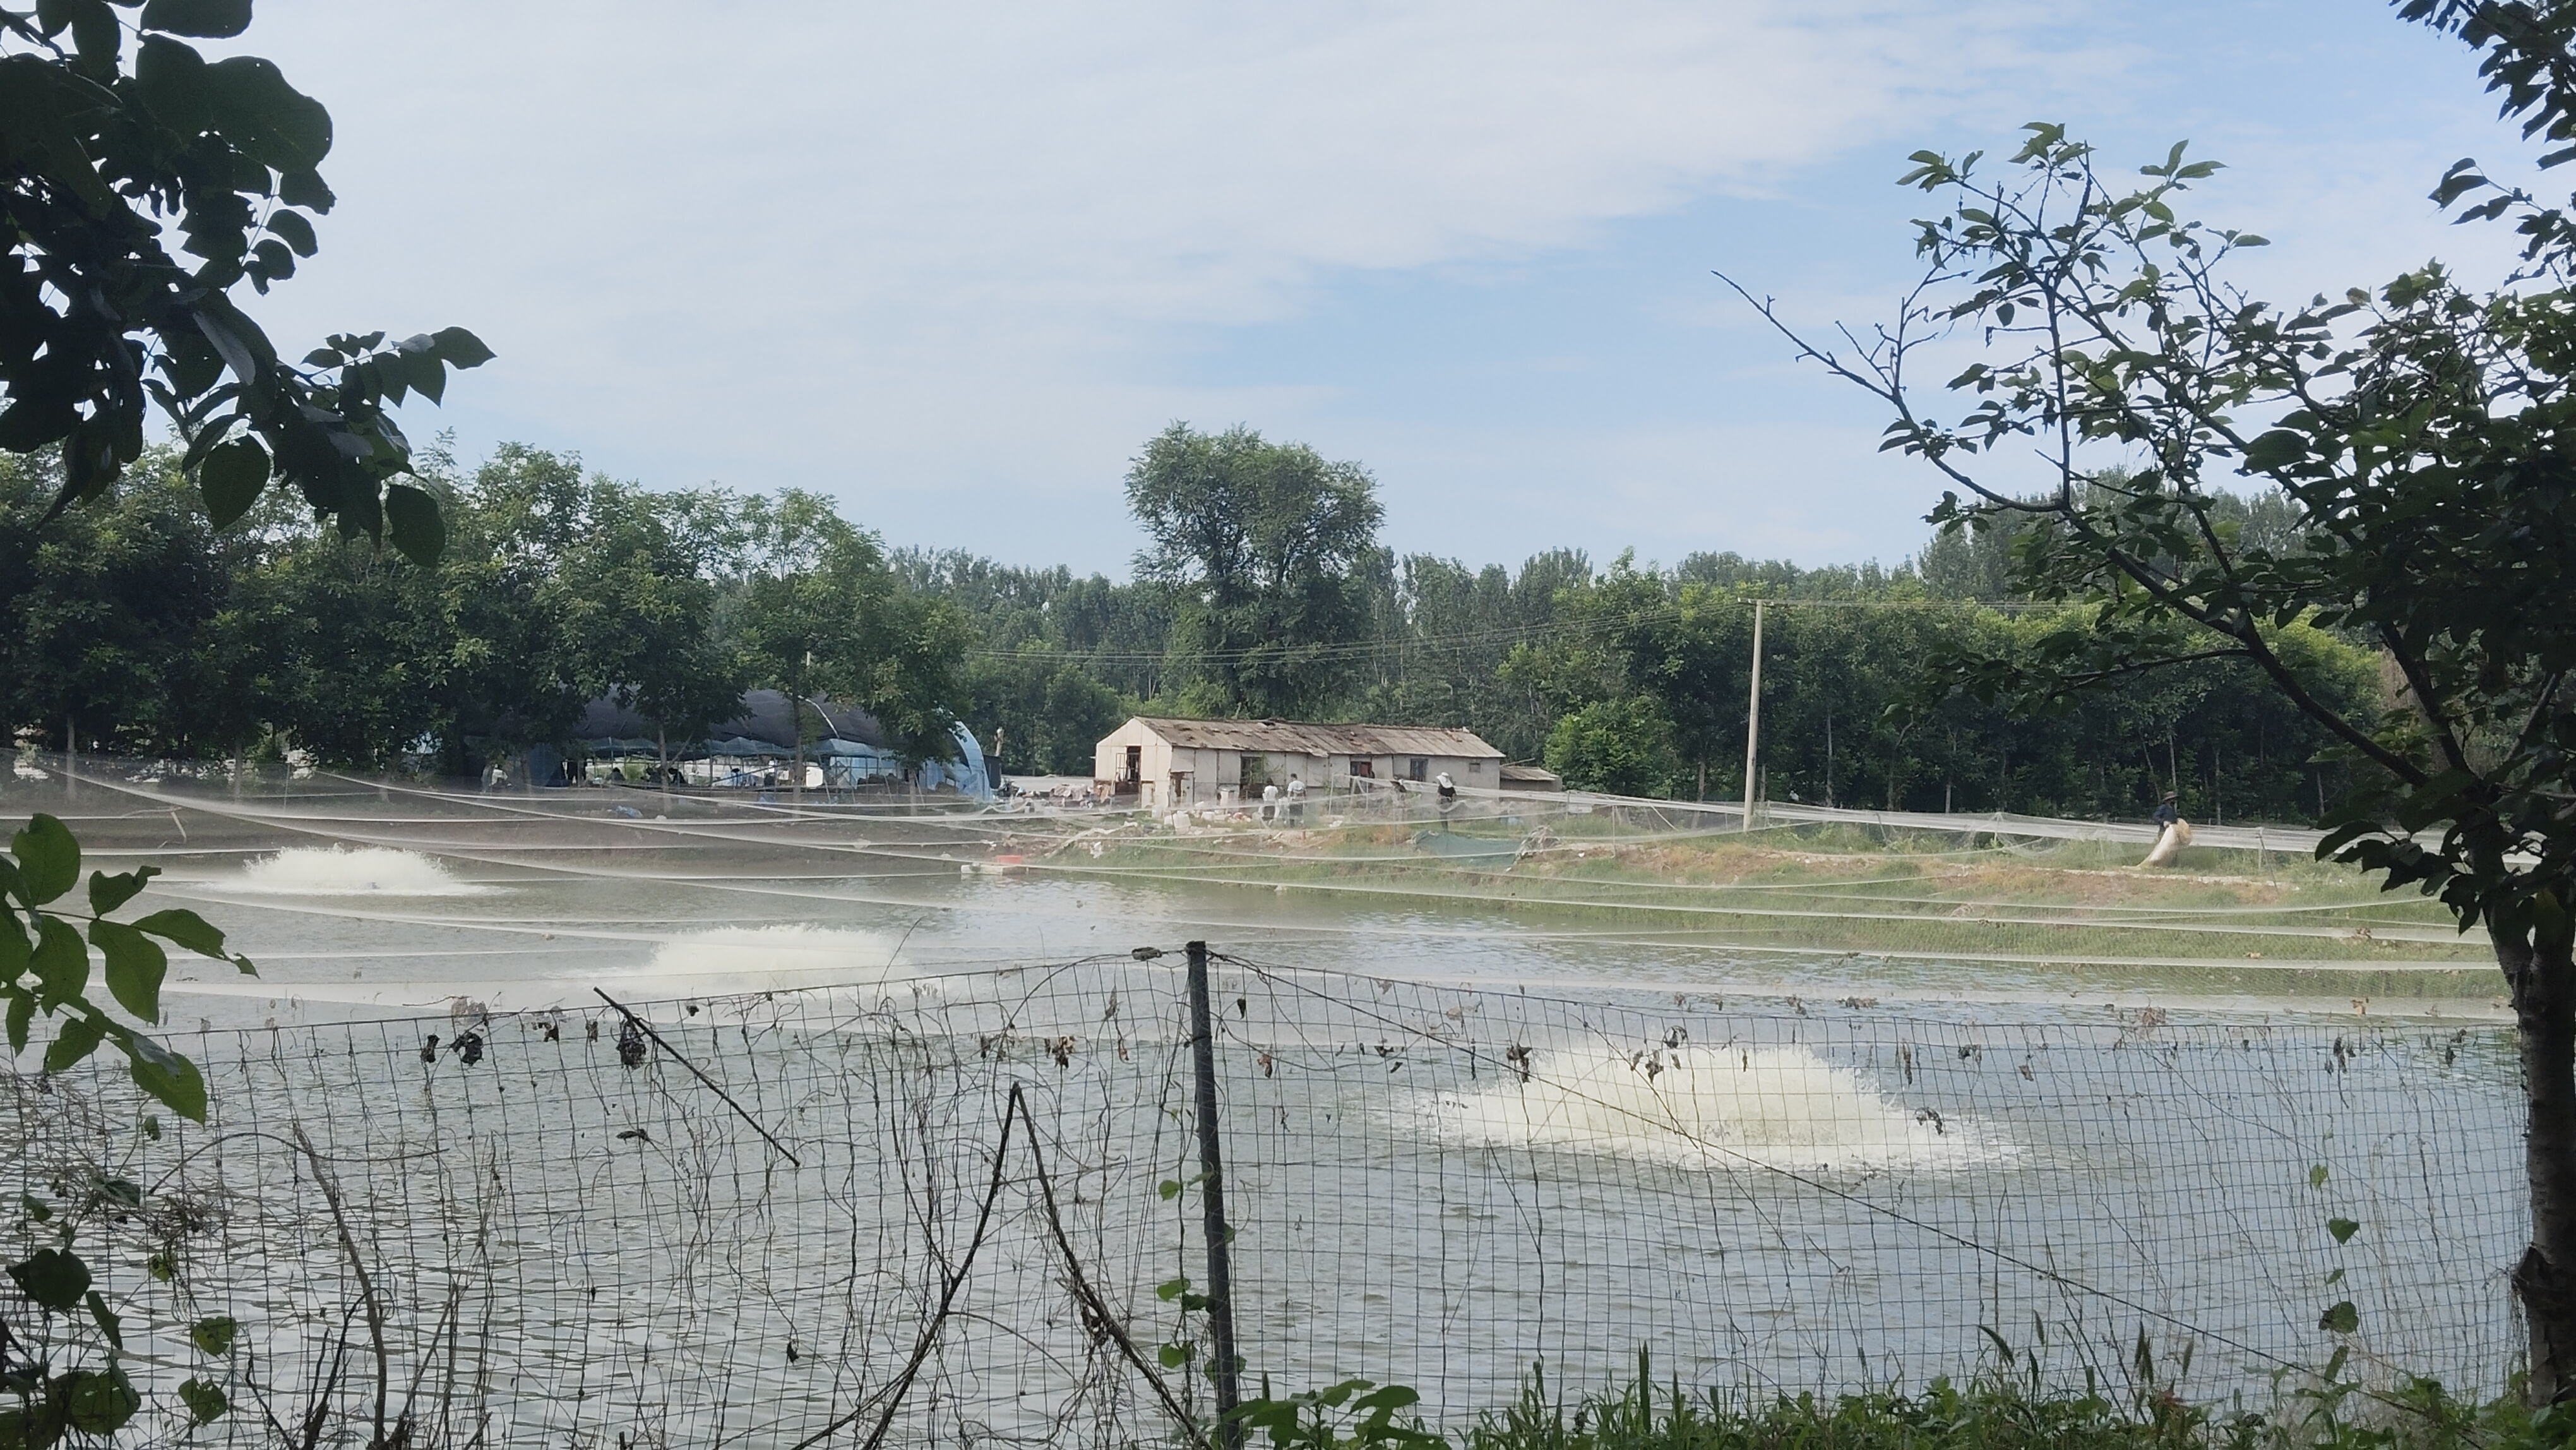
\includegraphics[width=0.85\textwidth]{fig1_pond_panorama.jpg}
\caption{北定福村鱼塘全景，可见增氧机运转与防鸟网覆盖}
\label{fig:pond_panorama}
\end{figure}

\section{平谷渔业现状与核心发现}

通过对四个村庄的调研数据交叉比对，我们提炼出以下八个核心发现。

\subsection{发现一：鱼价十年停滞，养殖户缺乏定价权}

四个村庄的养殖户给出的鱼价高度一致：每斤7\textasciitilde9元，且这一价格与十年前基本持平。而同期，饲料价格、电费、药品价格和人工成本均大幅上涨。

鱼价停滞的根本原因在于养殖户没有定价权。四个村庄的销售模式几乎完全相同：养殖户$\to$鱼贩子$\to$市场/网络。鱼贩子以7\textasciitilde9元/斤的价格收购后，在市场上以15\textasciitilde25元/斤的价格销售。马昌营村的养殖户老侯特别提到，"专业贩子收了以后挂网上卖"——贩子们在用养殖户不会使用的电商平台，赚取着养殖户赚不到的差价。

\subsection{发现二：从业人员全面老龄化，后继无人}

四个村庄的受访养殖户几乎全部在50岁以上。东双营镇的老赵、马昌营村的老侯，他们的子女均在外打工，过年才回一趟。没有人接班，是这个行业最根本的危机。

年轻人外流的深层原因并非单一的"嫌苦"，而是收入不稳定、劳动强度大、社会地位低、缺乏发展空间的综合结果。同样的劳动付出，在城市能获得更高的回报。

\subsection{发现三：销售渠道单一，利润被中间环节截取}

如表\ref{tab:sales}所示，四个村庄的销售渠道高度同质化，均以鱼贩子收购为主。

\begin{table}[H]
\centering
\caption{四个村庄销售渠道对比}
\label{tab:sales}
\begin{tabular}{ll}
\toprule
\textbf{村庄} & \textbf{主要销售渠道} \\
\midrule
北定福村 & 鱼贩子收购 \\
东双营镇 & 鱼贩子收购，无网络销售 \\
天井村 & 老板收货 + 微信本地销售（部分） \\
马昌营村 & 专业贩子收购，贩子挂网销售 \\
\bottomrule
\end{tabular}
\end{table}

天井村是唯一有"微信本地销售"的村庄，但也仅占部分比例。绝大多数鱼的流通仍然被中间商控制，养殖户在整个价值链中处于最底端。

\subsection{发现四：设备更新滞后，智能化程度极低}

增氧机是四个村庄唯一的"标配"设备，但状态参差不齐。马昌营村老侯的增氧机已使用六七年，早年有政府补贴，如今纯自费维护。自动投喂机单价3000\textasciitilde4000元，受访养殖户无人购置。水质检测靠试纸，鱼病靠肉眼观察，严重时才找"鱼大夫"。

东双营镇的老赵是唯一添置了部分智能设备的养殖户，并尝试了高价鱼种。但他的投入超过200万元，"纯利不高"四个字道出了投入与回报的不匹配。

\begin{figure}[H]
\centering
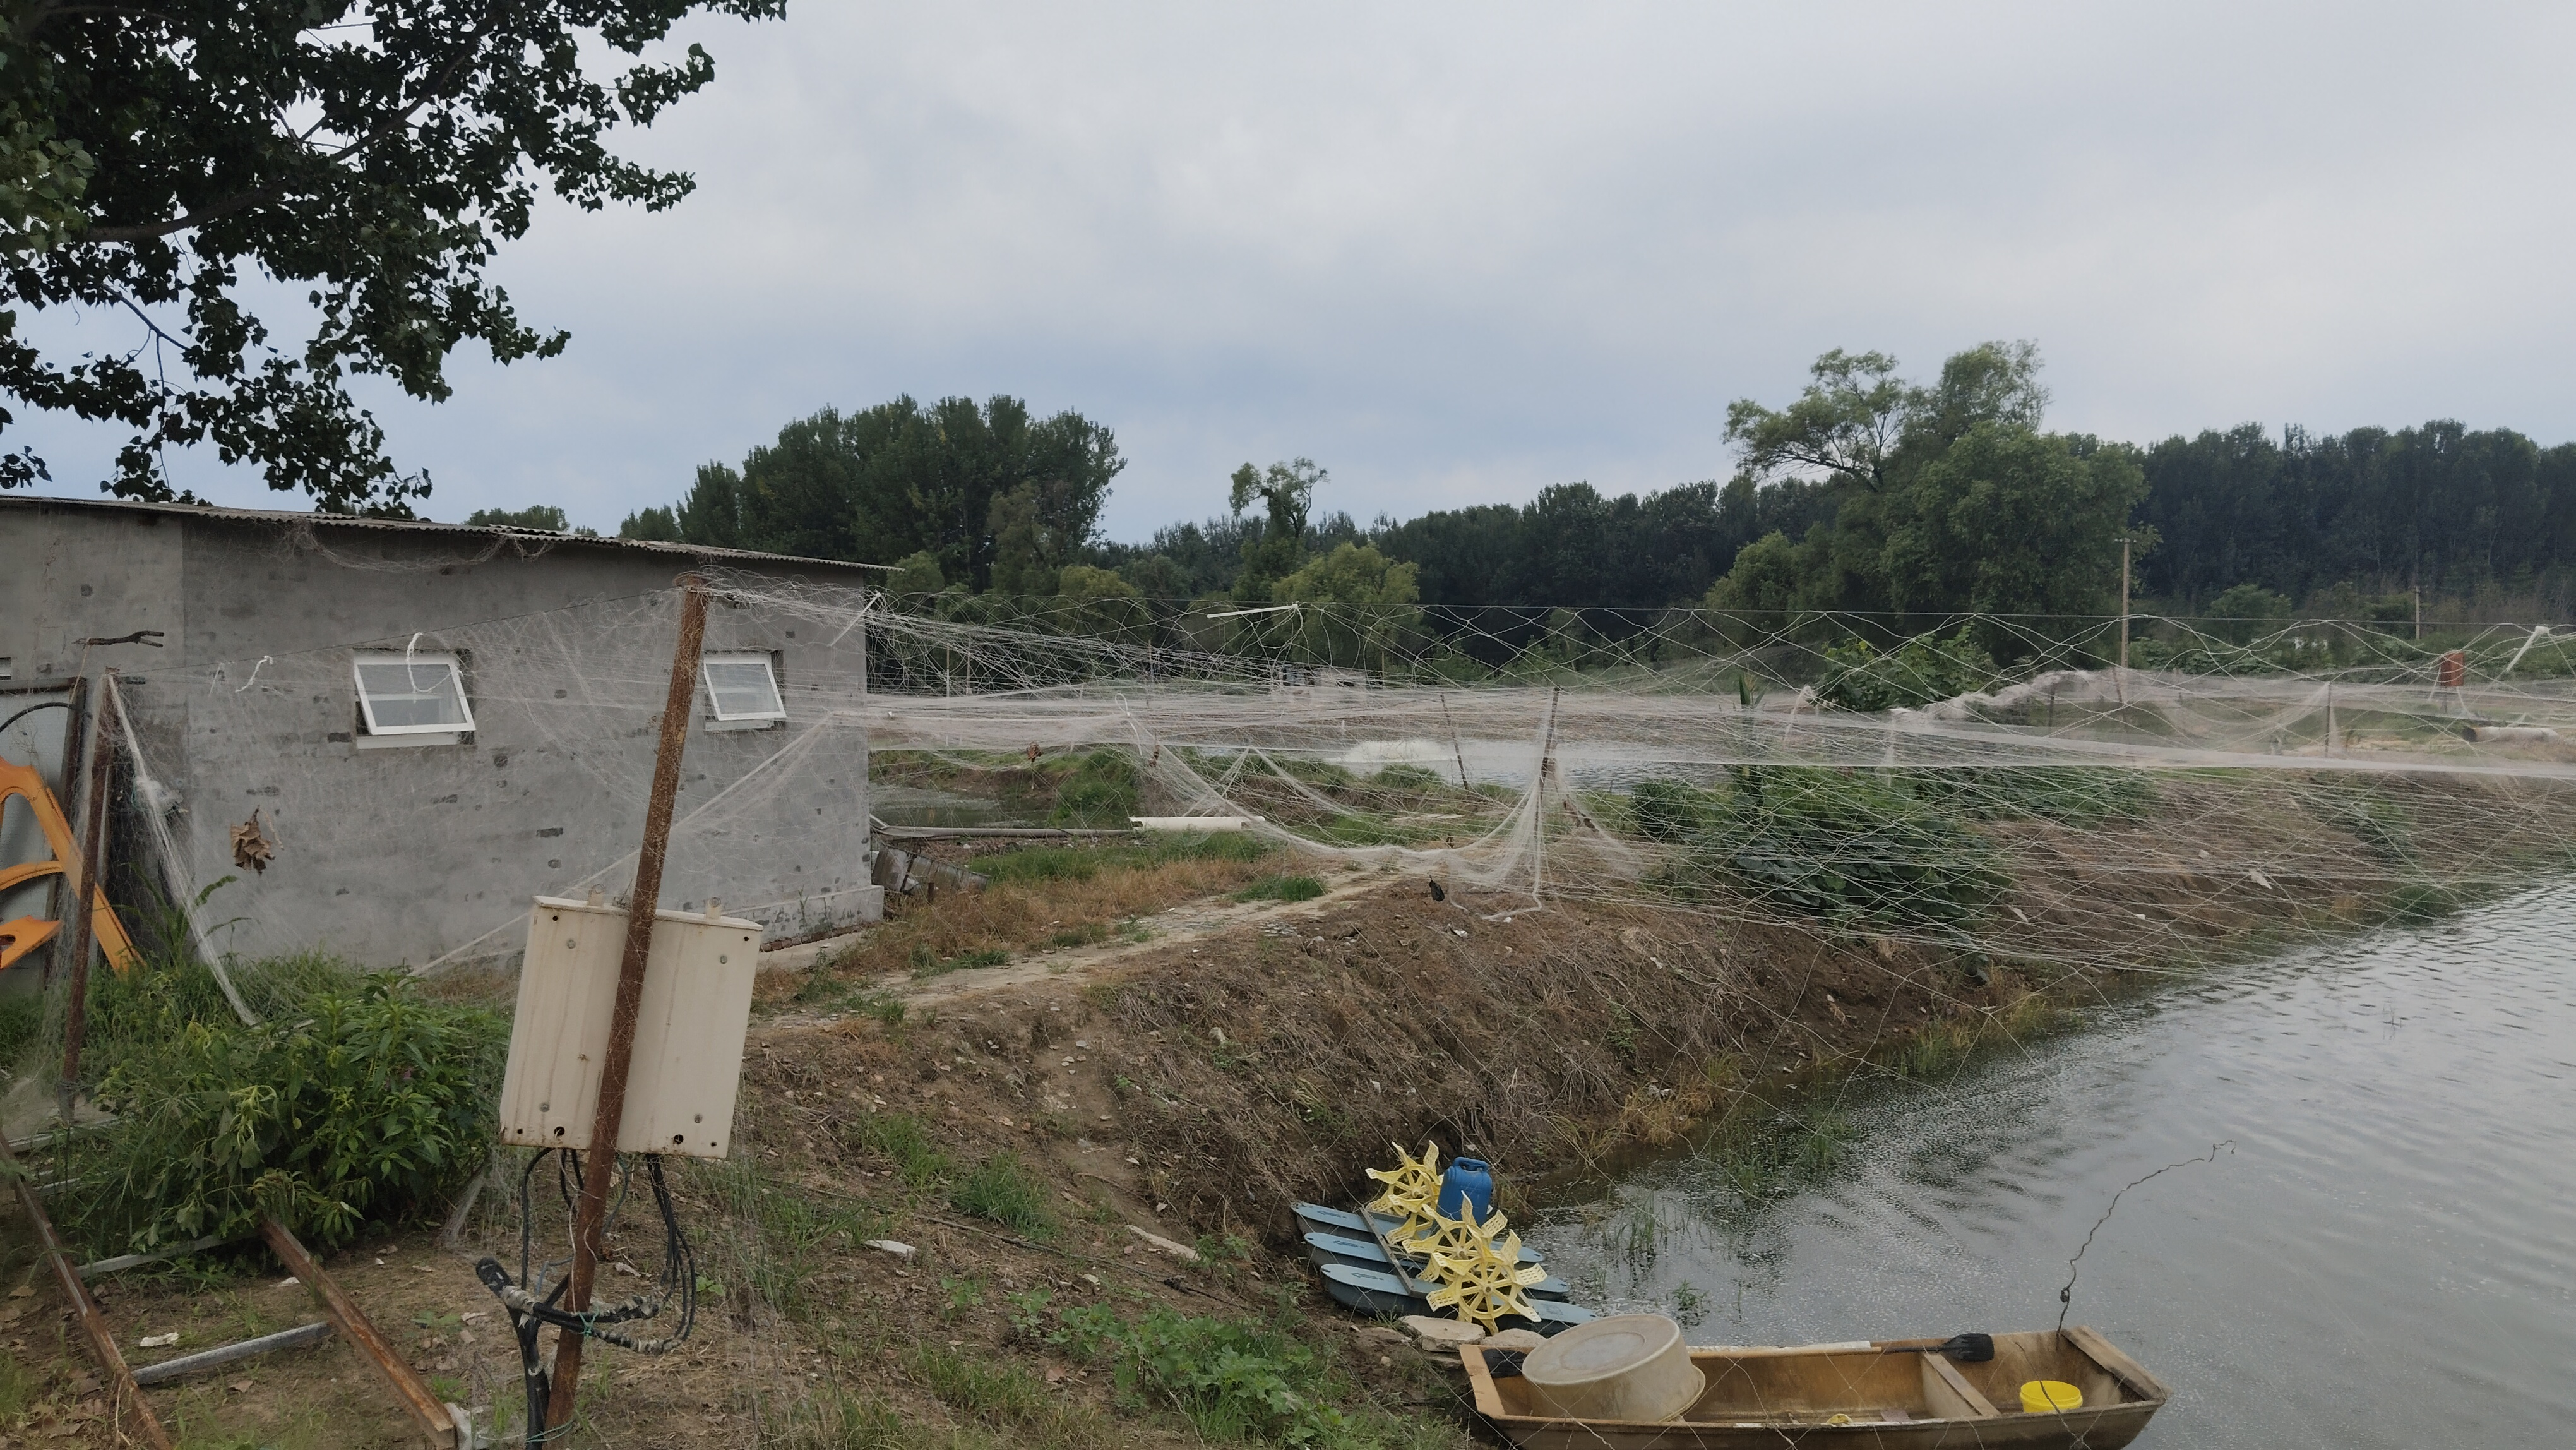
\includegraphics[width=0.85\textwidth]{fig2_boat_aerator.jpg}
\caption{鱼塘边的增氧机与简易木船，设备以基础型为主}
\label{fig:boat_aerator}
\end{figure}

\subsection{发现五：水质管理全凭经验，缺乏标准化方案}

"水质不好，一下雨就要调。"老侯的原话反映了当前水质管理的非标准化现状。天井村是唯一例外——该村的养殖户使用光合细菌调节水质，尾水排入藕池循环利用，形成了"鱼\textendash 藕"生态闭环。这一方法成本低、操作简单、效果显著，但其他三个村庄均未采用。

地下水质量一般、几乎不换水（东双营镇）、下雨后水质突变、渗水严重（天井村）等问题普遍存在。没有村庄具备系统的水质监测方案。

\subsection{发现六：北方养鱼的季节性困境}

"冬天水结冰，鱼卖不掉。"这是南方养鱼不存在的特有难题。平谷养殖户一年只能养一茬，有效销售期仅约半年，但增氧机运转、设备维护、土地租赁等成本全年持续。马昌营村亩产2000余斤，若按全年成本和半年销售窗口均摊，利润被大幅稀释。

\subsection{发现七：规划与落地之间存在鸿沟}

东双营镇35亩建设用地的旅游规划于2020年提出，构想是让城里人来钓鱼、吃鱼、体验渔村生活。五年过去，规划仍处于"不了了之"状态。资金不足、建设用地审批困难、缺乏运营经验、宣传渠道缺失等多重障碍叠加，导致"有想法、无落地"的困局。

\subsection{发现八：养殖户愿意改变，但缺乏路径指导}

这是我们最想强调的发现。老赵添置智能设备、尝试高价鱼种；老侯推动散户整合、追求规模化经营；天井村引进光合细菌、构建生态循环——他们并非固步自封，而是一直在用自己的方式寻找出路。但尝试是零散的、自发的，缺少系统的技术支持和市场指导。当被问及是否愿意将鱼挂到网上卖时，老侯的回答是："那敢情好。"

\begin{figure}[H]
\centering
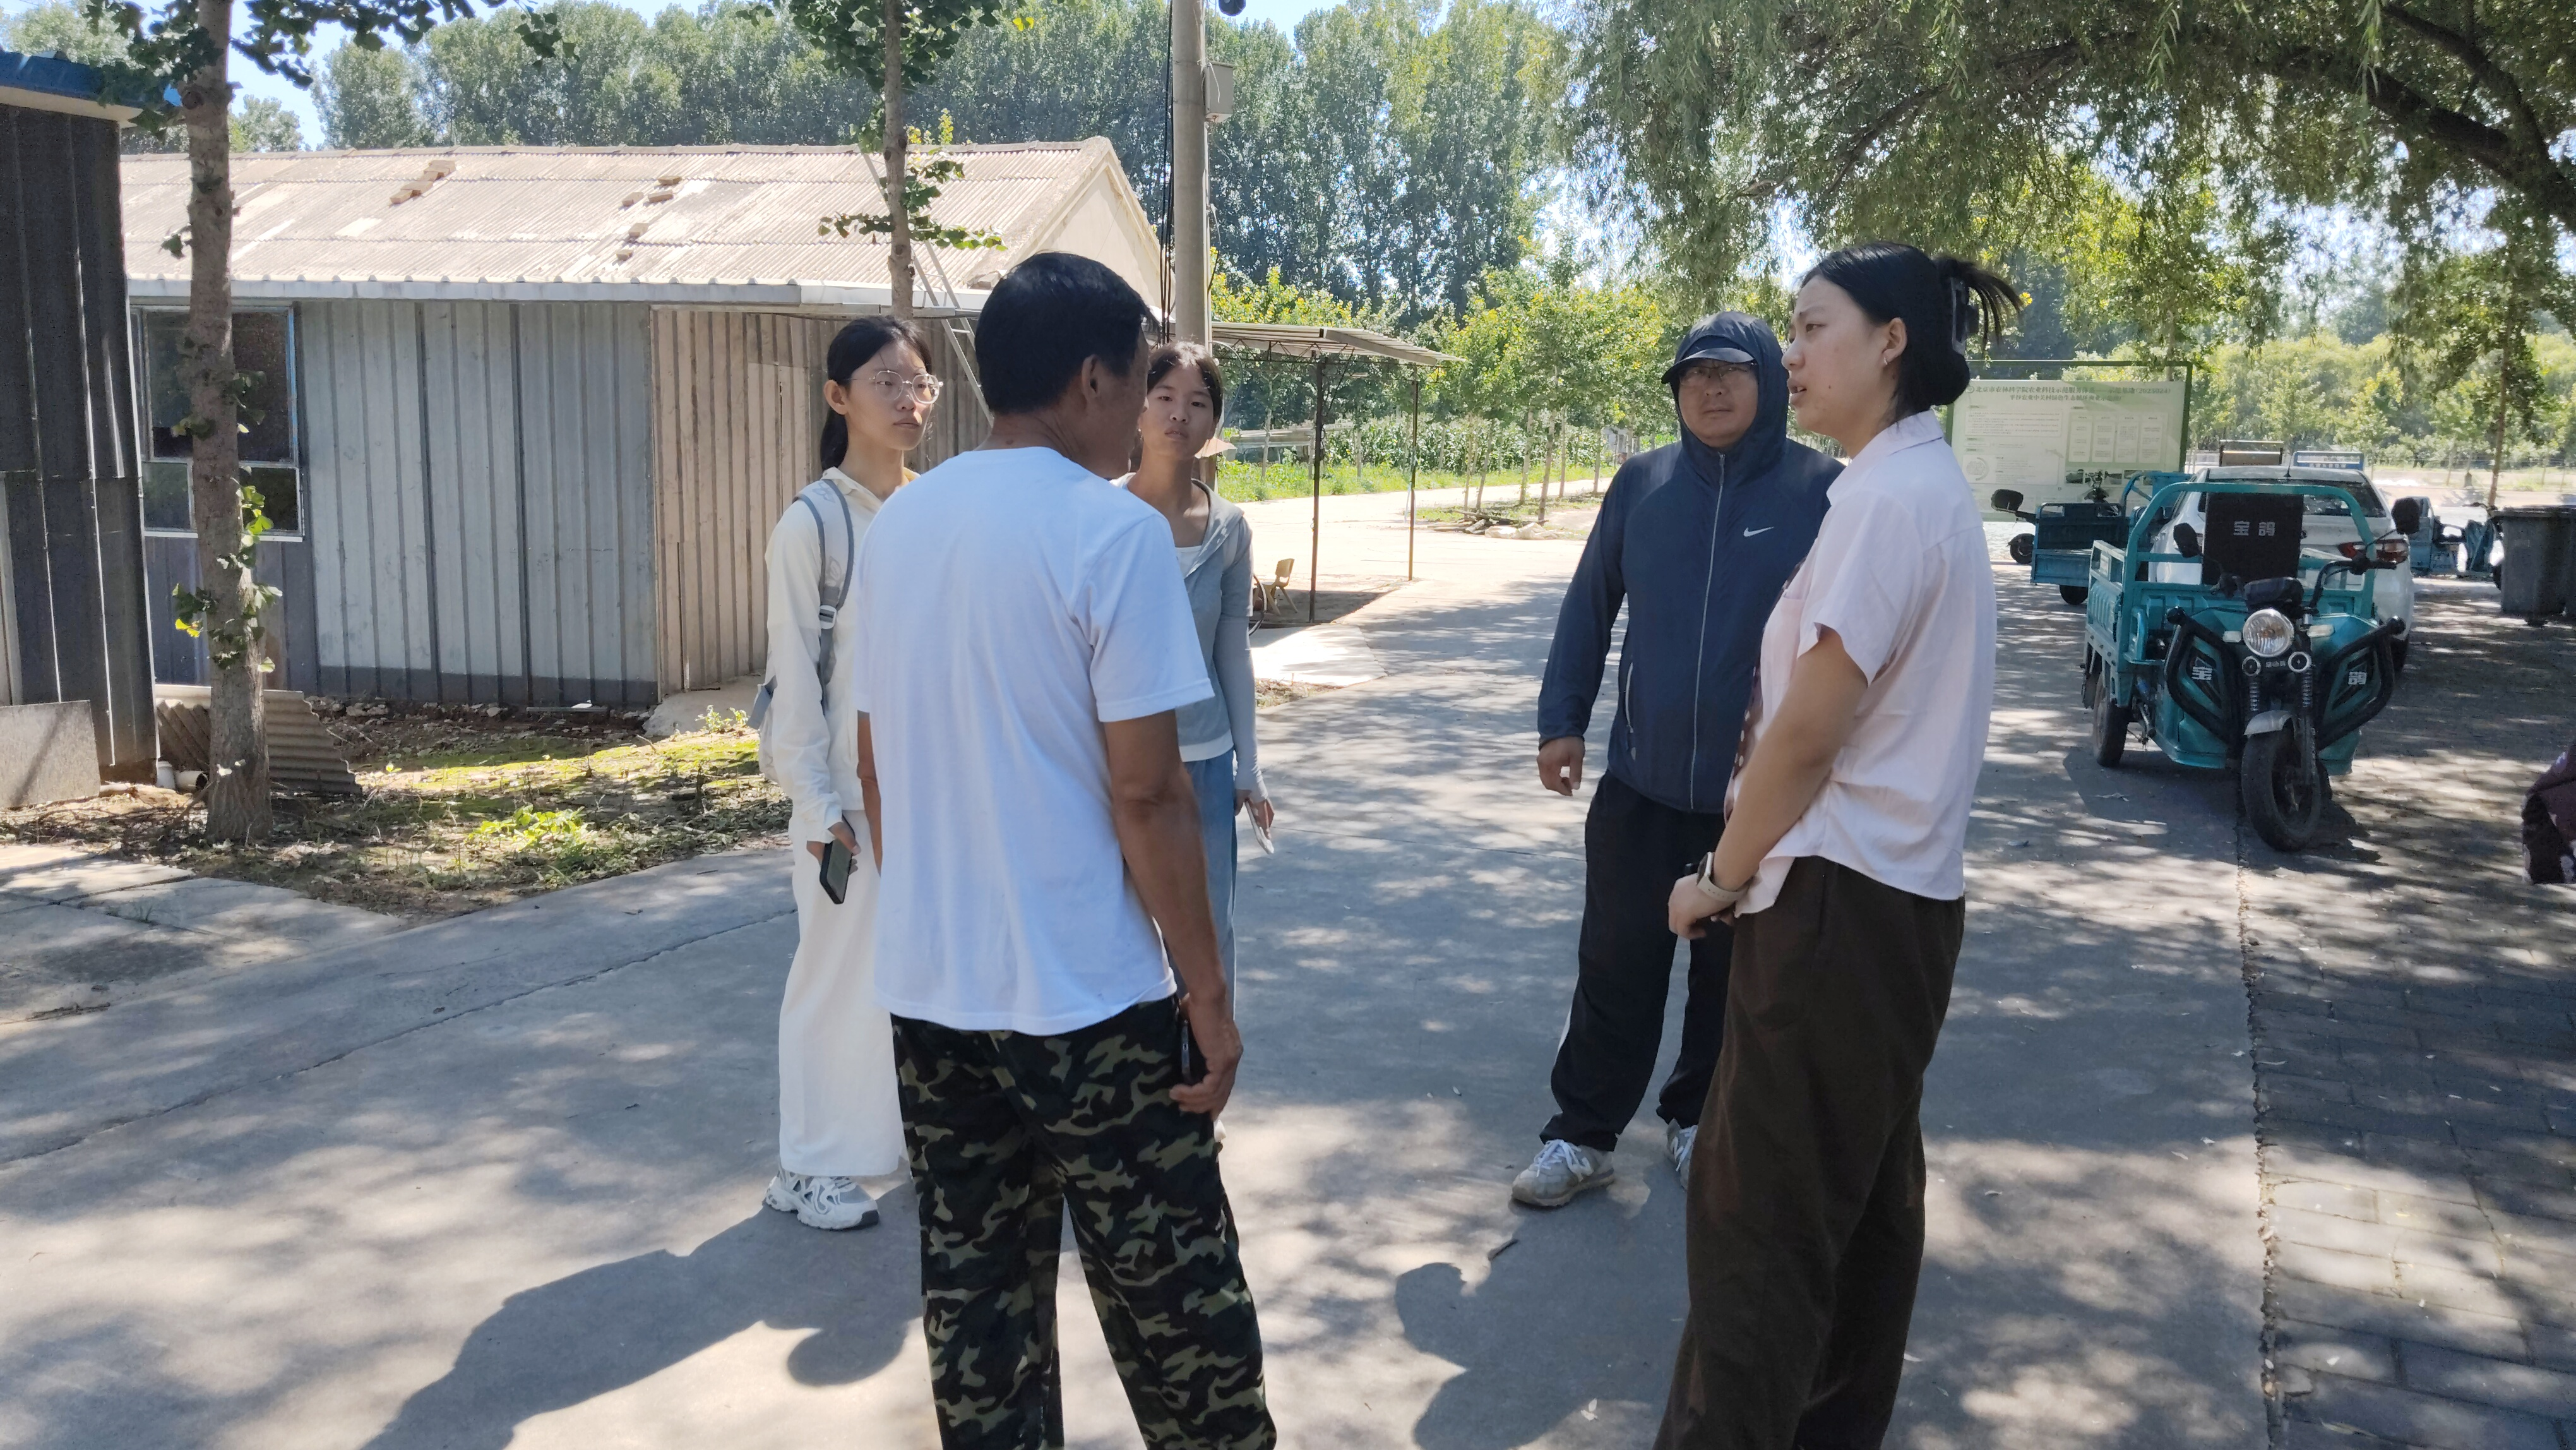
\includegraphics[width=0.75\textwidth]{fig10_interview.jpg}
\caption{调研队员与养殖户在村边进行访谈交流}
\label{fig:interview}
\end{figure}

\section{典型案例：天井村的生态养殖实践}

在四个村庄中，天井村的养殖模式最具参考价值，值得单独分析。

\subsection{技术方案}

天井村的生态养殖方案包含两个核心环节：

（1）\textbf{光合细菌水质调节}。向鱼塘投放光合细菌，利用其代谢活动增加水体含氧量、分解有机污染物、抑制有害藻类繁殖。光合细菌成本低廉、操作简单，不需要专门的设备或技术培训。

（2）\textbf{尾水循环利用}。鱼塘尾水不直接排放，而是引入相邻的藕池。藕池中的莲藕通过根系吸收水中的氮、磷等营养物质，实现水质的自然净化。净化后的水可回灌鱼塘，形成闭环。

此外，天井村还设置了两个专门的藕塘，在净化功能之外额外产出莲藕，增加了收入来源。

\subsection{推广价值}

天井村模式的核心优势在于\textbf{低成本}和\textbf{易复制}。光合细菌并非高技术产品，操作门槛低，普通养殖户经过简单培训即可掌握。尾水循环利用所需的藕塘用地可利用现有闲置坑塘，额外投入有限。若能将天井村的经验系统化、标准化，形成可复制的"平谷生态养鱼技术指南"，有望在全区乃至华北同类地区推广。

\section{数智化转型路径建议}

基于上述发现，本文提出以下四条转型路径。

\subsection{路径一：低成本智能投喂试点}

自动投喂机单价3000\textasciitilde4000元，看似不便宜，但可以进行经济性测算：以覆盖3\textasciitilde5个鱼塘计，一台投喂机每天节省人工投喂1\textasciitilde3小时，按3\textasciitilde5年使用寿命折算，日均成本仅2\textasciitilde3.5元。关键障碍不是"贵不贵"，而是"能不能先看到效果再投入"。

建议引入低成本试点方案，由高校或政府提供一台设备供一个鱼塘试用，用实际数据（省时、省料、鱼品一致性）说服养殖户。试点成功后，可通过合作社统一采购降低单价，或争取政府农机补贴政策支持。

\subsection{路径二：建立统一品牌与电商渠道}

平谷距北京城区1.5小时车程，"当日捕捞、当日送达"的生鲜电商模式完全可行。但不应让每个养殖户单独开店，而是建立\textbf{统一的品牌和运营平台}：由一个团队负责品牌设计、电商运营、物流配送，养殖户专注把鱼养好。

可参考"平谷大桃"的品牌化经验，打造"平谷鱼"区域公用品牌，通过微信公众号、视频号、抖音等新媒体平台进行内容营销。北京印刷学院实践队已建立"数智渔韵"公众号，为内容传播提供了初步渠道。

\subsection{路径三：推广天井村生态模式}

建议将天井村的"光合细菌+藕池循环"技术方案整理为标准化的操作手册，通过以下渠道推广：

（1）由区农业部门组织技术培训，邀请天井村养殖户现场教学；

（2）制作短视频教程，通过微信、抖音等平台传播；

（3）在示范鱼塘安装简易水质监测设备（pH计、溶氧仪），用数据验证生态模式的实际效果。

\subsection{路径四：发展休闲渔业}

北京常住人口超过2000万，周末休闲消费需求巨大。平谷已有桃花节、大桃采摘等成熟的乡村旅游IP，渔业可与之互补，形成"夏赏荷花秋品鱼"的全季旅游产品。

休闲渔业的关键不在于"让人钓鱼"，而在于提供完整的渔文化体验：拉网、喂鱼、水质检测、鱼塘科普等互动环节，结合养殖户故事的内容输出，打造"内容驱动"的体验式消费。东双营镇已规划的35亩建设用地可作为先期试点。

\section{讨论与反思}

本研究存在以下局限：一是调研时间较短（三天），且主要依赖访谈数据，缺乏量化问卷的支撑；二是样本量有限（四个村庄、十余位养殖户），结论的推广性需进一步验证；三是受限于调研团队的专业背景（印刷学院而非水产院校），对水质、鱼病等技术问题的分析深度不足。

尽管如此，本研究仍有其独特价值。作为一支以"数智传播"见长的团队，我们关注的不只是渔业技术问题，更是\textbf{信息鸿沟}和\textbf{数字鸿沟}如何制约传统产业升级的问题。养殖户说"那敢情好"的时候，我们看到的是一种真实的需求——他们需要的不是高科技本身，而是有人帮他们迈出从"不知道怎么变"到"知道怎么变"的第一步。

\section{结论}

本文通过对平谷区四个渔业村庄的实地调研，揭示了传统淡水养殖业面临的八大结构性困境：鱼价停滞、人才断档、渠道单一、设备落后、水质粗放、季节受限、规划搁浅、路径缺失。天井村的生态养殖实践证明，低成本、可复制的绿色转型路径是存在的。在此基础上，本文提出的智能投喂试点、统一品牌电商、生态模式推广、休闲渔业开发四条路径，构成了平谷渔业数智化转型的初步框架。

我们相信，每一尾鱼都值得一条更好的出路。这不仅是一个经济学命题，更是一个关于信息公平与数字包容的社会命题。

\vspace{1cm}
\begin{thebibliography}{99}

\bibitem{ref1} 国务院. 关于做好2023年全面推进乡村振兴重点工作的意见[Z]. 2023.

\bibitem{ref2} 农业农村部. 关于加快推进智慧渔业建设的指导意见[Z]. 2022.

\bibitem{ref3} 北京市平谷区人民政府. 平谷区"十四五"时期农业农村发展规划[Z]. 2021.

\bibitem{ref4} 李志刚, 张明. 中国淡水养殖业发展现状与趋势分析[J]. 中国渔业经济, 2023, 41(2): 15-23.

\bibitem{ref5} 王晓燕, 刘洋. 数字乡村建设背景下智慧渔业发展路径研究[J]. 农业经济问题, 2024(1): 88-96.

\bibitem{ref6} 陈建国. 北方淡水养殖季节性困境与对策[J]. 水产科技情报, 2022, 49(4): 45-50.

\bibitem{ref7} 张伟, 李芳. 生态循环渔业模式研究——以光合细菌应用为例[J]. 中国水产, 2023(6): 32-37.

\bibitem{ref8} 刘文. 乡村振兴背景下北京都市型渔业发展研究[D]. 中国农业大学, 2022.

\end{thebibliography}

\end{document}